\chapter{基于马尔科夫链的分布式聚类算法}

\section{引言}
列出目前分布式轨迹聚类或者说分布式聚类的处理方法,即传输原型向量或概率密度估计的方法。\\
阐述这样做的缺点,可以添加图。
分布不确定性和高维数据生成模型估计问题

\section{基于马尔科夫链的分布式聚类算法}

\sucsection{总体方案}
为了避免分布不确定性问题和高维数据生成模型轨迹问题,我们提出基于马尔科夫链的分布式聚类算法(MCD-Clustering)。为了避免分布不确定性问题,很自然想到直接传输属地数据概率分布模型参数到中心节点,这种方法在数据量大和数据维度低时使用,而一条具有500个二维坐标点的轨迹数据可以将其看做维度为1000的数据,此时估计数据概率分布模型的方法将不再使用,我们必须通过另外一种模型来估计轨迹数据的概率分布模型。因为每条轨迹各个点之间显然不是独立于彼此的,故当我们将轨迹数据看做是高维数据时,由于每条轨迹数据相邻点存在相关性,可以看做维度和维度之间存在相关性,我们基于这种认知提出使用马尔科夫链来模拟一簇相似轨迹的生成模型,于是提出了基于马尔科夫链的分布式聚类算法(MCD-Clustering)。方案大致流程如图\ref{ch4frame}所示解:

\begin{figure}[h]
	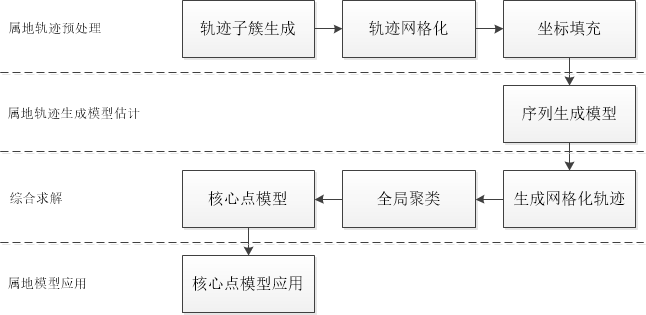
\includegraphics{ch4frame.png}
	\caption{MCD-Clustering 算法框架}
	\label{ch4frame}
\end{figure}

整个方案可以分为四个部分:属地轨迹预处理、属地轨迹生成模型估计、综合求解和属地模型应用。属地轨迹预处理,该阶段分为三个步骤:轨迹子簇生成、轨迹数据网格化和轨迹坐标填充。为了通过马尔科夫链能够更好的估计轨迹生成模型,首先对属地轨迹数据集进行聚类操作来得到多个轨迹子簇,我们假设一个子簇里面的轨迹大部分有着相同的轨迹形状。子簇生成后,针对每个子簇中的轨迹进行网格化操作,网格化的作用是通过更少数量的共用坐标点来表示子簇中所有轨迹中的坐标点。由于传感器在采样运动物体轨迹时存在不同物体速度的差异,所以经常会出现一条轨迹时间上相邻的坐标点在网格坐标中并不相邻,此时需要在这两个网格中不相邻的点以指定的策略补充一些坐标点,使得所有轨迹中时间上相邻的点在网格中也相邻。属地轨迹生成模型估计,通过马尔科夫链模型来模拟轨迹生成模型,利用属地轨迹数据集写出含有马尔科夫链参数的最大似然函数,利用最优化理论方法求得使最大似然函数取最大值的马尔科夫链参数。综合求解和属地模型应用,属地将求得的马尔科夫链参数传递给中心节点,中心节点通过这些参数重新生成轨迹坐标,利用重新生成的轨迹坐标作为全局聚类的输入,经过全局聚类输出若干簇心向量,将所有的簇心向量传递给各个计算节点,计算节点利用通过全局聚类计算出的簇心向量来对未知轨迹进行异常检测。\\

在进入方案具体流程之前,首先对常用符号进行定义。\\
假设计算节点的轨迹数据集记为D,轨迹数据集包含有n条轨迹,每条轨迹由m个坐标点构成,坐标点的维度为2,即:

\[
D=\left\{ t_1,t_2,...,t_n \right\} 
\\
t=\left\{ \left( x_1,y_1 \right) ,\left( x_2,y_2 \right) ,...,\left( x_m,y_m \right) \right\} 
\]

轨迹数据通过聚类算法产生的簇集合记为$C=\left\{ C_1,C_2,...,C_k \right\} $,其对应的簇心向量记为$\mu =\left\{ \mu _1,\mu _2,...,\mu _k \right\} $。


\subsection{属地轨迹预处理}

属地轨迹预处理分为三个阶段:轨迹子簇生成、轨迹数据网格化和轨迹坐标填充。\\

轨迹子簇生成阶段主要通过聚类算法来实现,本节选择k-means++算法进行聚类,通过聚类算法生成的轨迹子簇记为集合C,其中聚类中使用的距离度量与第三章定义的距离一样,假设两条轨迹a和b,则轨迹a和b之间的距离为:

\[
\text{Dist}\left( \text{a},\text{b} \right) =\frac{1}{m}\sum_{i=1}^m{\sqrt{\left( a_{x}^{i}-b_{x}^{i} \right) ^2+\left( a_{y}^{i}-b_{y}^{i} \right) ^2}}
\]

k-means++聚类在选择k值时需要聚类评价指标来评判不同k值下的聚类效果,这里采用内部指标DI来衡量,DI表达式如式\ref{DI}所示。\\

k-means++初始化操作如下:

\begin{algorithm}[H]
	 \KwData{样本集$D=\left\{t_1,t_2,...,t_n\}\right\}$,簇个数K}
	 \KwResult{簇心向量$\mu=\left\{\mu_1,\mu_2,...,\mu_K\}\right\}$}
	 从数据集D中随机初始化1个样本,将其作为第一个簇的簇心$\mu={\mu_1$}\;
	 \Repeat{k=2,3,...,K}{
	 	R=D-$\mu$
	 	\For{$t_i$ in R}{
	 		计算$P(x_i)$,$P\left( t_i \right) =\omega \sum_{\mu _i\in \mu}{\left( t_i-\mu _i \right) ^2}$,其中$\omega$是归一化系数\;\\
	 	}
	 	按照R集合中所有点的概率分布选出$\mu_k$,将其加入集合$\mu$\;\\
	 }
	 \caption{kmeanspp_initialization}
\end{algorithm}

轨迹子簇生成的具体流程如下:

\begin{algorithm}[H]
	 \KwData{样本集$D=\left\{t_1,t_2,...,t_n\}\right\}$,簇个数K,阈值S}
	 \KwResult{簇划分$C=\left\{C_1,C_2,...,C_K\}\right\}$,簇心向量$\mu=\left\{\mu_1,\mu_2,...,\mu_K\}\right\}$}
	 K=2\;\\
	 kmeanspp_initialization\(D,K\)\;
	 C,$\mu$=kmeans\(D,K\)\;
	 $DI_K$=DI(C)\;
	 flag=true\;
	 \Repeat{flag}{
	 	K=K+1\;
	 	kmeans_initialization\(D,K\)\;
	 	C,$\mu$=kmeans\(D,K\)\;	
	 	DI_K=DI(C)\; 
	 	\If{$DI_K-DI_{K-1}\leqslant S$}{
	 		flag=false\;
	 	}	
	 }
	 \caption{轨迹子簇生成流程}
\end{algorithm}

轨迹子簇生成后,针对每个子簇进行网格化。原始轨迹数据中的坐标点在二维连续空间上取值,将轨迹数据网格化后,轨迹所有坐标点在二维离散网格空间取值。最简单的网格化则是将二维连续空间中的点坐标取整,即将二维连续空间映射到由所有整数构成的坐标形成的二维离散网格空间,如图\ref{gridization}所示。

\begin{figure}[h]
	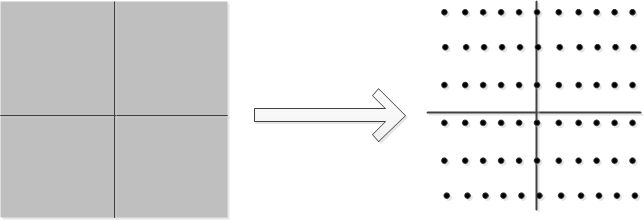
\includegraphics{gridization.png}
	\caption{空间网格化}
	\label{gridization}
\end{figure}

对于轨迹数据可以采用同样的方法对其进行网格化,网格化规则可以通过下面式子表示:

\[
f\left( x \right) =\left\{ \begin{array}{c}
	sign\left( x \right) *\left( \lfloor x \rfloor +1 \right) \,\,if\,\,|x-\lfloor x \rfloor |>0.5\\
	sign\left( x \right) *\left( \lfloor x \rfloor -1 \right) \,\,if\,\,|x-\lfloor x \rfloor |\leqslant 0.5|\\
\end{array} \right. 
\\
\varPhi \left( \left( x,y \right) \right) =\left( f\left( x \right) ,f\left( y \right) \right) 
\\
g\left\{ \left( x_1,y_1 \right) ,\left( x_2,y_2 \right) ,...,\left( x_l,y_l \right) \right\} =\left( x_1,y_1 \right) \,\, if\,\,\left( x_1,y_1 \right) =\left( x_2,y_2 \right) =...=\left( x_l,y_l \right) 
\]

其中,sign(x)表示实数x的符号。通过上式规则对轨迹中的每一个坐标点进行网格化,图\ref{gridization}展现了轨迹经过网格化后的效果,图\ref{originaltrajectory}表示原始轨迹数据,图\ref{gridedtrajectory}表示网格化后的轨迹数据。网格化对轨迹数据的精度造成了一定程度的影响,但是完全不影响其对轨迹形状的刻画。

\begin{figure}[h]
\subfigure[]{
\label{originaltrajectory}
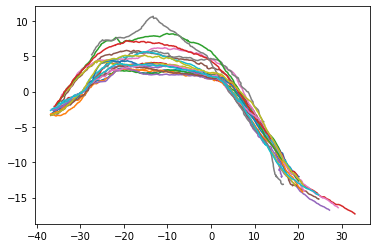
\includegraphics[width=6.77cm]{originaltrajectory.png}}
\subfigure[]{
\label{gridedtrajectory}
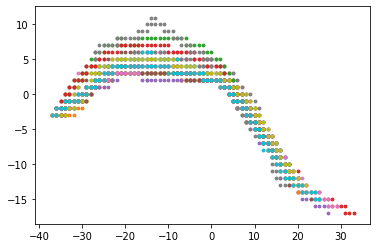
\includegraphics[width=7.04cm]{gridedtrajectory.png}}
\caption{轨迹网格化前后对比}
\label{gridization}
\end{figure}


由于传感器在采样运动物体轨迹时存在不同物体速度的差异,所以经常会出现一条轨迹时间上相邻的坐标点在网格空间中并不相邻,此时需要在这两个网格中不相邻的点之间通过指定的操作填充一些坐标点,使得所有轨迹中时间上相邻的点在网格空间中也相邻,这种保证了网格空间数据相邻性的操作称之为轨迹数据填充操作。假设一条网格化后的轨迹数据记为$g=\left\{ \left( x_1,y_1 \right) ,\left( x_2,y_2 \right) ,...,\left( x_l,y_l \right) \right\} $,轨迹数据填充操作流程如下:

\begin{algorithm}[H]
 	\KwData{一条网格化的轨迹$g=\left\{ \left( x_1,y_1 \right) ,\left( x_2,y_2 \right) ,...,\left( x_l,y_l \right) \right\} $}
 	\KwResult{轨迹数据填充后的轨迹数据$\hat{g}=\left\{ \left( x_1,y_1 \right) ,\left( x_2,y_2 \right) ,...,\left( x_s,y_s \right) \right\} $}

	 \Repeat{i=1,2,...,l-1}{
	 	\If{$x_i==x_{i+1}$ && $|y_i-y_{i+1}|>1$}{
	 		s = sign($y_{i+1}-y_{i}$)
	 		在坐标$(x_i,y_i)$后面填充坐标$(x_i,y_i+s),(x_i,y_i+2*s),...,(x_i,y_{i+1}-s)$
	 	}
	 	\ElseIf{$y_i==y_{i+1}$ && $|x_i-x_{i+1}|>1$}{
	 		s = sign($x_{i+1}-x_i$)
	 		在坐标$(x_i,y_i)$后面填充坐标$(x_i+s,y_i),(x_i+2*s,y_i),...,(x_{i+1}-s,y_{i})$
	 	} 
	 	\ElseIf{$|x_i-x_{i+1}| \geqslant 1$ && $|y_i-y_{i+1}| \geqslant 1$}{
	 		xs = sign($x_{i+1}-x_i$)
	 		ys = sign($y_{i+1}-y_{i}$)
	 		在坐标$(x_i,y_i)$后面填充坐标$(x_i+xs,y_i),(x_i+xs,y_i+ys)$
	 		\While{假设最后填充的坐标$(x_t,y_t)$不满足:$x_t==x_{i+1}$ || $y_t==y_{i+1}$ || ($|x_t-x_{i+1}|==1$ && $|y_t-y_{i+1}|==1$) }{
	 			在坐标$(x_t,y_t)$后面填充坐标$(x_t+xs,y_t),(x_t+xs,y_t+ys)$
	 		}
	 		\If{$x_t==x_{i+1}$ && $|y_t-y_{i+1}|>1$}{
	 		s = sign($y_{i+1}-y_{t}$)
	 		在坐标$(x_t,y_t)$后面填充坐标$(x_t,y_t+s),(x_t,y_t+2*s),...,(x_t,y_{i+1}-s)$
	 		}
	 		\ElseIf{$y_t==y_{i+1}$ && $|x_t-x_{i+1}|>1$}{
	 			s = sign($x_{i+1}-x_t$)
	 			在坐标$(x_t,y_t)$后面填充坐标$(x_t+s,y_t),(x_t+2*s,y_t),...,(x_{i+1}-s,y_{t})$
	 		}
	 		\ElseIf{$|x_t-x_{i+1}|==1$ && $|y_t-y_{i+1}|==1$}{
	 			s = sign($x_{i+1}-x_t$)
	 			在坐标$(x_t,y_t)$后面填充坐标$(x_t+s,y_t)$
	 		}
	 	}
	 }
	 \caption{轨迹数据填充操作}
\end{algorithm}



\subsection{属地轨迹生成模型估计}

\subsection{综合求解和属地模型应用}
稀疏表示
聚类距离

\section{实验与分析}

\section{本章小结}
